\section{Introduction}

The rapid advancements in large language models (LLMs) have been driven by innovations in model architectures~\cite{NIPS2017_3f5ee243} and training paradigms~\cite{radford2019language, NEURIPS2020_1457c0d6}. Moreover, with the guidance of scaling laws~\cite{kaplan2020scaling}, models prove to become stronger with increasing number of parameters or training data. Tokenization, the process of converting raw text into discrete tokens as the input and output of the model, is recently found relevant to scaling laws, where larger models deserve larger vocabulary and achieve better performance under the same training cost~\cite{tao2024scaling}. In fact, expanding the input vocabulary incurs almost no additional computational cost, whereas expanding the output vocabulary significantly increases the training overhead for smaller models. Thus, it is natural to consider decoupling the input and output vocabularies for separate investigations. Our research is fundamentally based on this idea.

\begin{figure}
    \centering
    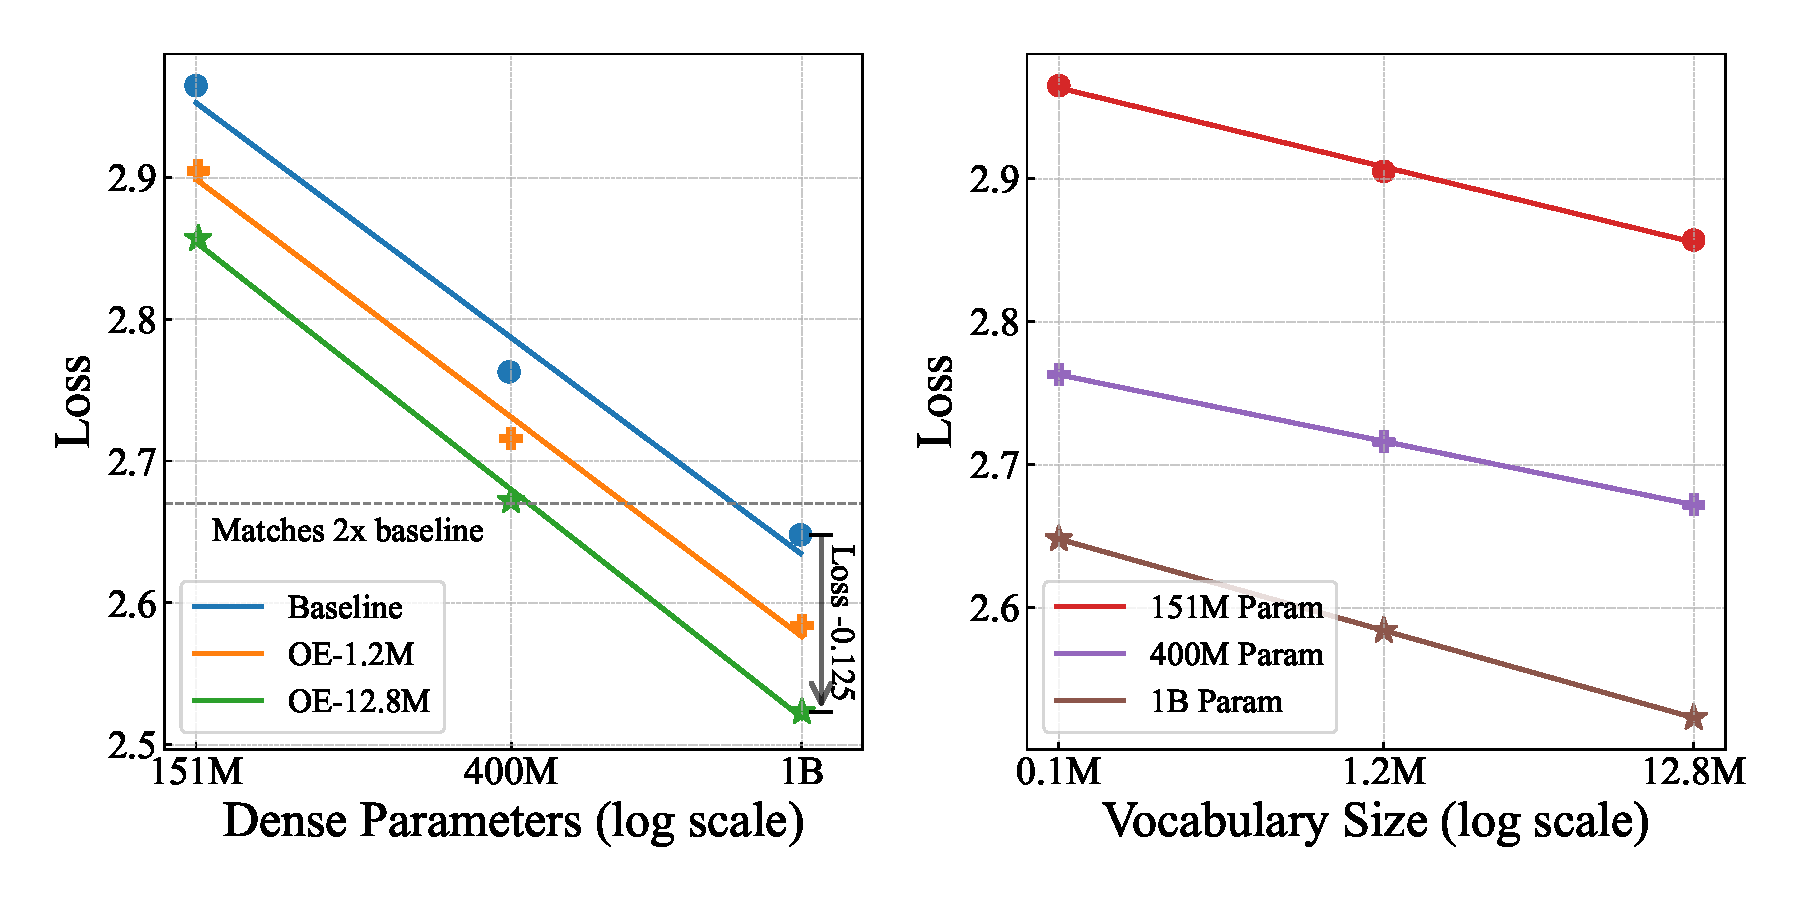
\includegraphics[width=\linewidth, trim=15 5 15 5, clip]{figures/olmo2_model_size_scale.pdf}
    \caption{Scaling trend for Over-Encoded models and baselines on OLMo2. We plot the loss with 400B tokens' training. For over-encoding, input vocabulary size is extended from 0.1 to 1.2 and 12.8 million ($12\times$ and $128\times$ larger than baseline), referred to as OE-1.2M and OE-12.8M. We observe OE-12.8M with 400M parameters matches the baseline with 1B parameters.}
    \label{fig:model_size_scaling}
\end{figure}


Starting with synthetic experiments on context-free grammar modeling, we systematically analyze the effects of token granularity and vocabulary size on models of varying scales. Firstly, it is revealed that larger tokenizers improve the performance of larger models while introducing challenges for smaller ones, which is consistent with previous studies. Furthermore, once the input and output vocabulary is decoupled, we find that scaling up input vocabulary solely keeps improving model, while larger output vocabulary may be harmful to smaller models. This insight motivates the development of Over-Tokenized Transformers, which decouple the encoding and decoding vocabularies to achieve greater flexibility and performance gains. 

Specifically, we introduce Over-Encoding(OE), which utilizes large hierarchical $n$-gram input vocabulary. As shown in \figref{fig:model_size_scaling}, our method improves the model scalability by a significant margin. Increasing the input vocabulary size by 128$\times$, our 400M model matches the training loss of a 1B baseline with no additional training cost (see left panel). More interestingly, we observe a strong log-linear relationship between the input vocabulary size and model performance, \ie, exponentially increasing the input vocabulary size consistently results in a linear decrease in loss (see right panel). These findings represent a new dimension in scaling laws and also indicate embedding parameters as a new scalable sparse dimension. Moreover, we propose the concept of Over-Decoding(OD), which leverages larger output vocabulary to provide more fine-grained supervision. We typically treat multi-token prediction methods~\cite{gloeckle2024better,deepseekai2024deepseekv3technicalreport} as approximations of OD. Combining OE and OD together, we build Over-Tokenized Transformer, which shows greater potential than apply either OE or OD solely.

Although introducing a large amount of embedding parameters for OE, the training and inference cost barely increases, as embedding parameters are used in an extremely sparse manner. In practice, we propose efficient engineering solutions to mitigate the computational and memory challenges introduced by large vocabularies, resulting an additional training overhead less than 5\%. 

Through this work, we aim to bridge the gap between tokenizer design and model scaling, positioning tokenization as a critical factor in the continued evolution of large language models.

\section{Related Work}

\subsection{Tokenization Design}
Tokenization is a critical component in the development of large language models (LLMs). Established methods such as Byte-Pair Encoding (BPE)~\cite{sennrich2015neural} and Unigram Language Models~\cite{kudo2018subword} have been widely adopted to create subword vocabularies that balance sequence length and vocabulary size. Recently, alternative paradigms have been proposed to address the computational inefficiencies of byte-level models~\cite{xue-etal-2022-byt5,clark2022canine,tay2022charformer,yu2023megabyte}. For instance, MegaByte~\cite{yu2023megabyte} combines byte-level modeling with patching by first predicting patches and then predicting bytes within each patch, improving processing efficiency. However, its performance at scale remains inferior to that of tokenizer-based approaches. Building on this concept, 
In this work, our findings suggest that applying $n$-gram embeddings on top of BPE expands the vocabulary size, improving model capability, while BLT~\cite{pagnoni2024bytelatenttransformerpatches} also has the same finding on byte-level models.

\subsection{Scaling Vocabulary}
\citet{huang21f_interspeech} firstly explores recurrent neural networks with scalable $n$-gram embedding table, where modular hashing is used to control vocabulary size. \citet{roy2022ngrammeraugmentingtransformerslatent} further augments the Transformer architecture with $n$-grams that are constructed from a discrete latent representation of the text sequence. Recent empirical studies have systematically investigated the relationship between vocabulary size and model performance. \citet{tao2024scaling} demonstrates that expanded vocabularies enhance both training efficiency and model performance, particularly in larger architectures. Building on these findings, we argue that vocabulary size research should separately consider embedding (input) and unembedding (output). While embedding incurs only lookup costs, unembedding introduces computational costs that scale with vocabulary size. More importantly, we find that input and output vocabularies exhibit distinct scaling behaviors, underscoring the need for independent scaling strategies to optimize model design. Moreover, \citet{liu2024infinigram} revisits $n$-gram language modeling at massive scale, proposing an $\infty$-gram model trained on 5 trillion tokens, which achieves competitive performance and can effectively complement neural LMs to reduce perplexity.

\subsection{Multi-Token Prediction}
Multi-Token Prediction (MTP)~\cite{stern2018blockwise,qi2020prophetnet,gloeckle2024better} has advanced the field of next-token prediction through the introduction of auxiliary objectives for simultaneous multi-token prediction. This methodology shares fundamental principles with our $n$-gram modeling framework, where multi-token prediction can be theoretically formulated as an approximation of $n$-gram unembedding utilization (over-decoded models). In our work, we further compare the effectiveness of MTP and over-encoded models, demonstrating that the performance gains from MTP and over-encoded models are complementary and can be combined to achieve even greater improvements. 
